\documentclass[aps,letterpaper,11pt]{revtex4}

\usepackage{graphicx}
\usepackage{float}
\usepackage{verbatim}
\usepackage{amsmath}
\usepackage{amssymb}

\newcommand{\labno}{11}
\newcommand{\labtitle}{Calculating the distance a rocket travels using the impulse-momentum and Work-Energy theorem }
\newcommand{\authorname}{Kevin Truong}
\newcommand{\professor}{Dr. Melanie Lutz}
\newcommand{\classno}{Physics 006}
\newcommand{\labpartners}{Sean Casey, Kevin Castillo, and Dulce Payan}
\newcommand{\submitdate}{May 12,2017}

\begin{document}

\begin{titlepage}
\begin{center}
\hspace{-136mm}\boxed{{\Large \textsc{Lab No. \labno}}}\\\vspace{30mm}
{\Large \textsc{\labtitle} \\ \vspace{4pt}}
\rule[13pt]{\textwidth}{1pt}\\ \vspace{150pt}
{\large By: \authorname \\ \vspace{10pt}}
Lab Partners: \labpartners \\
Instructor: \professor \vspace{10pt} \\
Solano Community College\\ \classno \\ \vspace{10pt}
\submitdate
\end{center}
\end{titlepage}

\section{Abstract}

In this experiment both the impulse-momentum theorem and the work-energy theorem were used to calculate the total height that the rocket traveled. The impulse-momentum theorem was used during the thrust stage of the rocket's flight, when the impulse of thrust due to the engine ignition went against the impulse due to the drag forces and the impulse of the weight of the rocket to shoot the rocket upward. The work-energy theorem was used to calculate the height that the rocket traveled during the coast stage. The summation of the heights found in these two stages was the total height that the rocket achieved during its flight. The theoretical calculation for the height achieved was 113.78m while the experimental height achieved was 126.71m. The percent error was 11.39\%. Some factors that might have affected this may have been the environment such as the wind blowing the rocket to obtain a greater height.

\section{Introduction}

A Rocket's engine must have enough impulse to overcome the impulse due to drag and impulse do to gravity to accelerate away from earth. In real rockets, the thrust of the engine is strong enough and lasts long enough to get the rocket out of earth's atmosphere. In this experiment the engine didn't have enough thrust or last long enough to reach that point. Therefore there was a stage when the rocket was accelerating upward due to the thrust of the engine (thrust stage) and a stage when the rocket just coasted to a peak height (coast stage). During the thrust stage the impulse-momentum theorem was used to calculate the height achieved during this stage:

$$ J = \bar{F}\Delta t$$ 

and 

$$ J = \Delta p$$

During the coast stage the work-energy theorem was used to calculate the distance traveled during this stage:

$$ W_{other} + Energy_1 = Energy_2$$

In this experiment drag forces were taken into account to make sure that the calculations were as accurate as possible.

\section{Experimental Details}

Equipment for this experiment includes an assembled wizard rocket, rocket launching stand, rocket engine, timer, and protractor gun. The assembled wizard rocket was decorated and was prepared for lift off. The rocket launching stand kept the rocket in place, so that it could lift off. The rocket engine provided the rocket with thrust and lifted the rocket off the stand and into the sky. The timer was used to calculate the time of the rocket from its initial position to the end of the coast stage. The protactor gun was used to calculate the angle from the user's perspective from where the rocket releases its smoke indicating the end of the coasting stage. Four protractor guns were used at the end of the field to get a more accurate angle. 

This experiment utilizes the impulse-momentum theorem to calculate the total distance the rocket traveled after being launched. The rocket's flight was broken up into two stages, a thrust stage and a coast stage. The thrust stage is the initial ignition of the engine until the engine runs out of "fuel;" the impulse-momentum theorem will be used in this stage to calculate the distance traveled during this stage.  The coast stage is when the engine runs out of "fuel" but has momentum due the impulse of the engine and continues to rise until the drag force and the force due to gravity slows the rocket down to a final peak height; conservation of energy will be used to solve for the distance traveled during this portion. 

\begin{center}
\underline{Diagram 1}\\
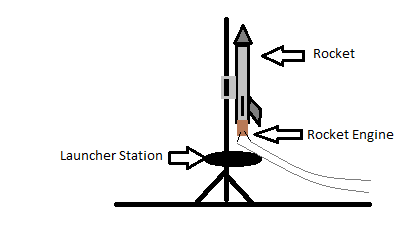
\includegraphics[width = 4in]{Setup.png}\\
\textit{Diagram 1: Setup For the Rocket Launch}\\
\end{center}

\section{Results and Analysis}

When calculating the total distance that the rocket travels during its flight, it's necessary to break the flight into two different stages. One stage when the impulse created by the thrust of the engine causes the rocket to move upward to some height and a second stage when the engine runs out of fuel and the rocket coasts, slowing down due to gravity and drag forces, to some other height. With the summation of these two heights, it's possible to calculate the total height that the rocket travels during its flight. 

\subsection{Thrust Stage}

The distance, $d_1$, achieved during the thrust stage was calculated using the impulse-momentum theorem. Impulse is equal to the change in momentum of the object, impulse is also equal to the average force on the object over some amount of time. The total impulse on the rocket during the thrust stage is the impulse caused by the thrust of the engine minus the impulse caused by the weight of the rocket minus the impulse caused by the drag forces. 

$$ J_T = J_E - J_D - J_w$$

Impulse is also: $J = \bar{F}\Delta t$. The impulse of the thrust was obtained by collecting data on the engine when ignited and affected the force sensor. The impulse due to the drag forces was calculated using the equation $J = \bar{F}\Delta t$ where $\bar{F}$ was given to be 0.35N and $\Delta t$ was found during the launching of the rockets using timers from the moment the rocket launched until the puff of smoke came out. For the impusle due to gravity the force was just the average weight of the rocket, it's important to average the mass of the rocket throughout the flight because as the engine uses "fuel" it will have less and less mass, so a good estimate of the average mass is looking at the mass prior to launch and after all of the fuel is dispersed from the engine; the $\Delta t$ is the same time that was used for the impulse of the drag force.

$\therefore J_T = J_E - f_D\Delta t_1 - m_Tg\Delta t_1$, where $m_T = (\frac{m_0+m_1}{2})$ and $m_0$ is the mass of the rocket with the engine with full fuel and $m_1$ is the mass of the rocket once most of the fuel is used at the end of the thrust stage.

impulse is also equal to the change in momentum($\Delta p$) in a body. The momentum right before launch is zero because the velocity of the rocket is zero, but once all of the fuel is depleted there is some velocity and some mass, so there is momentum. 

$$ \therefore m_1v_1 = J_E - f_D\Delta t_1 - m_Tg\Delta t_1$$

Solving for $v_1$:

$$ v_1 = \frac{J_E - f_D\Delta t_1 - m_Tg\Delta t_1}{m_1}$$

\begin{center}
\underline{Diagram 2}\\
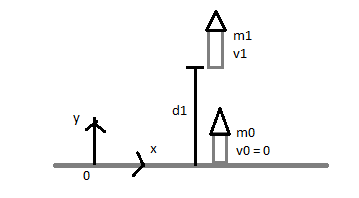
\includegraphics[width = 4in]{CalculatingD1.png}\\
\textit{Diagram 2: Thrust stage of the rocket. Showing that in the first state there is no velocity prior to launch and there is some momentum at $d_1$.}
\end{center}

A big assumption that was made during the experiment was, the thrust of the rocket would cause the rocket to have a constant acceleration which would allow us to use the kinematic equation for constant acceleration.

$d_1$ expressed as a kinematic equation:

$$ d_1 = d_0 + v_{0y}t + \frac{1}{2}a_yt_1^2$$

Looking at diagram 2, $d_0$ is at the origin and the initial velocity at the origin is zero, so the equation can be simplified:

$$ d_1 = \frac{1}{2}a_{y}t_1^2$$



Since acceleration was assumed to be constant acceleration can also be written as the slope of the velocity vs. time graph: $a_y = \frac{v_1}{t_1}$

$$ \therefore d_1 = \frac{1}{2}(\frac{v_1}{t_1})t_1^2 = \frac{1}{2}v_1t_1$$

Using the equation that we arrived from earlier with the equation we just derived: 

$$ d_1 = \frac{1}{2}v_1t_1 $$ 

and

$$  v_1 = \frac{J_E - f_D\Delta t_1 - m_Tg\Delta t_1}{m_1}$$

The new equation for $d_1$:

$$ d_1 = \frac{1}{2}(\frac{J_E - f_D\Delta t_1 - m_Tg\Delta t_1}{m_1})\Delta t_1$$

This is the theoretical equation that will be used to calcualte the distance traveled during the thrust stage.

\subsection{Coast Stage}

After most of the fuel in the rocket engine is used, there was no more impulse from the thrust causing the rocket to acceleration upward. Therefore the drag forces and force due to gravity is causing the rocket to slow down to a stop to a final height $d_2$.

\begin{center}
\underline{Diagram 3}\\
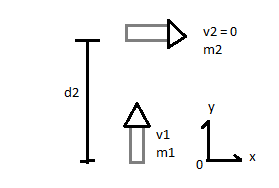
\includegraphics[width=3in]{CalculatingD2.png}\\
\textit{Diagram 3: Coast stage of the rocket, the first state is when the rocket engine runs out of most of its fuel and the only force acting on the rocket is drag forces and the weight of the rocket causing the rocket to slow down to a stop, which would be the second state.}
\end{center}

The work-energy theorem can be used:

$$ W_{other} + GPE_1 + KE_1 = GPE_2 + KE_2$$

where the first state is when the rocket begins in coast stage, and the second state is when the rocket reaches the peak of it's flight.

Looking at diagram 3, there is no GPE in state one and there is no KE in state two because the velocity at the peak is zero. The work done by other forces would be only the drag force, it's working against the motion of the rocket, so the work done would be negative:

$$ -f_Dd_2 + \frac{1}{2}m_1v_1^2 = (\frac{m_1+m_2}{2})gd_2$$

solvind for $d_2$ and simplifying:

$$ d_2 = \frac{m_1v_1^2}{(m_1+m_2)g + 2f_D}$$

but from the thrust stage $v_1$ was found to be: 

$$  v_1 = \frac{J_E - f_D\Delta t_1 - m_Tg\Delta t_1}{m_1}$$

subbing this into the equation for $d_2$:

$$ d_2 = \frac{(J_E-f_D\Delta t_1-m_Tg\Delta t_1)^2}{[(m_1+m_2)g+2f_D]m_1}$$

where $m_T$ = $\frac{m_0+m_1}{2}$

\subsection{Calculations Using Data}

In the equation for $d_1$ and $d_2$ there are many unknowns that need to be found: 

\begin{center}
\underline{Table 1}\\
\begin{tabular}{|c|c|}
\hline
Variables & Data\\
\hline
$m_0$ (The rocket's mass with the engine and all the fuel) & 0.0298 kg\\
\hline
$m_1$ (The rocket's mass when the thrust stage ends) & 0.0267kg\\
\hline
$m_2$ (the rocket's mass when the coast stage ends) & 0.024kg\\
\hline
$f_D$ (The drag force on the rocket on the Wizard model) & 0.350N\\
\hline
$J_E$ (The average impulse of the thrust due to the engine) & 2.222N*s\\
\hline
$t_1$ (The time duration of the rocket during the thrust stage) & 0.899s\\
\hline
\end{tabular}
\end{center}

With the data found during the experiment $d_1$ and $d_2$ can be found:

$$ d_1 = \frac{1}{2}(\frac{J_E - f_D\Delta t_1 - m_Tg\Delta t_1}{m_1})\Delta t_1$$

$$ d_2 = \frac{(J_E-f_D\Delta t_1-m_Tg\Delta t_1)^2}{[(m_1+m_2)g+2f_D]m_1}$$

$$d_1 = \frac{1}{2}(\frac{2.222N*s - (0.350N)(0.899s) - (\frac{0.0298kg+0.0267kg}{2})(9.8\frac{m}{s^2})(0.899s)}{0.0267kg})(0.899s) $$

$$ d_2 = \frac{(2.222N*s-0.350N(0.899s)-(\frac{0.0298kg + 0.0267kg}{2})(9.8\frac{m}{s^2})(0.899s))^2}{[(0.0267kg+0.024kg)(9.8\frac{m}{s^2})+2(0.350N)](0.0267kg)}$$

$$ d_1 \approx 27.92m$$

$$ d_2 \approx 85.86m$$

solving for the total theoretical values: 

$$ d_t = d_1 +d_2$$

$$ d_t = 113.78m$$

The theoretical height that the rocket should travel is 113.78m.

When the rocket was actually launched the experimental height that was achieved was 126.71m. The data (In the Appendix) given only had the height of the first run. The best height would have been the average heights of the two runs, adding the height from the first launch with the heigh achieved in the second launch divided by two. However, only one height from one of the launches was provided. 

The \% error between the theoretical height and the experimental height can be calculated using: 

$$ \% error = |\frac{theoretical-experimental}{theoretical}|*100\%$$

$$ \% error = |\frac{113.78m - 126.71m}{113.78}|*100\% = \boxed{11.36\%}$$

\section{Discussion} 

The peak height achieved during the experiment was 126.71m, compared to the theoretical height there was a 11.36\% error. it's important to note that during the thrust stage acceleration was assumed to be constant for the simplicity of the calculation, but this assumption could be a source of error. Also the environment could have been a source of error, the winds may have push the rocket upward or downward. During the launch it was very windy, so this is a very likely cause for error.

\section{Appendix}

(Attached to this report is the raw data collected and organized by Dr.Lutz)

\section{References}

\hspace{-6.5mm}
Rocket Science Physics 06 Lab, Dr. Melanie Lutz\\



\end{document}
